\documentclass[UTF8,a4paper,twocolumn,10pt]{ctexart}
\usepackage[left=1.65cm,right=1.65cm,top=1.8cm,bottom=1.8cm,columnsep=0.65cm]{geometry}
\usepackage{amsmath,amssymb,array,booktabs,graphicx,tabularx,xurl}
\usepackage[numbers,sort&compress]{natbib}
\usepackage{hyperref}
\hypersetup{hidelinks}
\setlength{\emergencystretch}{3em}
\setlength{\parindent}{2em}
\setlength{\parskip}{0pt}
\renewcommand{\figurename}{图}
\renewcommand{\tablename}{表}
\renewcommand{\refname}{参考文献}

\title{面向可审计实体--关系抽取的来源保持型证据门控知识图谱增强方法}
\author{Xuelin Hu，Xiaoqin Fu，Youjing Fu，Jingchao Wang\thanks{通信作者：Jingchao Wang，static@zut.edu.cn}，\\
Ruishen Liu，Charles Jumaa Katila，Pengming Hu}
\date{}

\begin{document}
\maketitle

\begin{abstract}
图谱增强抽取可以检索有用的关联，但被检索到的关联不一定是当前句子明确陈述的事实，流畅的生成结果也往往难以追溯到支持它的源文本。本文提出一种保持来源信息的证据门控框架，将图谱引导的候选生成与最终输出接受明确分离。系统仅从训练标注构建知识图谱，为经 QLoRA 适配的 Qwen3-4B 抽取器提供有界的概念和关系提示；随后通过确定性的跨度重建、实体接受和关系验证，仅保留能够链接到源文本且类型兼容的断言。本文在 ADE 和 CoNLL04 上采用统一的严格字符跨度协议，并同时报告数据集的标签与句长分布。实验表明，PGE 在两个基准上的关系 F1 均高于匹配的纯源文本生成器，而且每个接受决定均可检查；这一关系优势在两个数据集的两次追加训练中，以及排除 CoNLL04 训练--测试精确文本重叠后仍然保持。结果表明，受控图谱增强能够在提升关系抽取性能的同时，保留明确的源文本链接和可检查的接受决策，从而为安全敏感场景中的人机协同知识构建提供可审计的技术基础。
\end{abstract}

\noindent\textbf{关键词：}实体与关系抽取；知识图谱；来源追踪；证据锚定

\section{引言}
结构化信息抽取把非结构化文本转化为可检索的实体、类型化关系和下游知识对象。在安全相关应用中，仅输出形式正确的三元组并不足够，分析人员还需要知道模型识别了哪个文本片段、哪个句子支持该关系，以及最终断言经过了哪些转换。药物不良反应抽取直观地体现了这一需求：即便模型正确识别了药物和不良反应，若凭空建立二者关系，仍会形成误导性记录。

神经实体与关系模型已经为识别任务提供了有效方案\cite{li2022ner,eberts2020spert}。生成模型可以跨标签体系复用统一的结构化输出格式，但语言流畅并不保证预测对象受到输入支持\cite{ji2023hallucination}。当错误三元组被写入知识图谱并供后续检索或推理使用时，其影响可能超出最初的源句。

知识图谱能够提供类型化领域先验\cite{hogan2021kg}，检索增强则可在不把全部知识固化到模型参数中的情况下使用这些先验\cite{lewis2020rag}。然而，训练句中出现过的关系只能提示模型寻找某类关联，不能证明该关系在新句中成立；图谱还可能返回当前样本自身的标注，或者泄漏跨划分的重复内容。因此，关键问题不仅是图谱上下文能否提高召回率，还包括其资格、影响和接受过程能否被控制与审计。

本文构建分阶段架构：纯源文本抽取（SOE）、精确锚点抽取（EAE）和高召回图谱抽取（HRGE）形成输入条件匹配的生成分支；确定性关系验证器检查引用、类型和源证据；实体门控依据分支一致性、源匹配锚点或已验证关系端点接受候选；最终的来源门控抽取（PGE）仅组合被接受的实体及其验证关系。本文提出的是一种来源约束的“图谱增强—断言接受”协议：图谱记录可以影响候选生成，但只有得到源文本支持且类型兼容的候选才能进入最终断言，从而将检索上下文的权威边界与接受语义分离并设为可检查对象。

实验聚焦 ADE\cite{gurulingappa2012ade} 与 CoNLL04\cite{roth2004conll}。ADE 是含两类实体和一类关系的药物安全相关任务；CoNLL04 是含四类实体和五类有向关系的通用领域对照。两者均为英文句级输入，并分别训练与评估，因此本文不涉及跨数据集零样本迁移。主要贡献包括：（1）来源约束的图谱增强策略，将图谱资格判定与候选生成分离，只使用训练标注、排除仅由当前样本支持的提示并隔离精确重叠文本；（2）明确的断言接受语义，通过源跨度重建、类型化端点检查和确定性证据门控，将候选转换为可审计输出并记录接受或拒绝原因；（3）结合匹配的纯源文本比较、追加运行、配对不确定性、规则合规性、消融和重叠敏感性分析的双基准实证研究。

\section{相关工作}
\subsection{联合实体与关系抽取}
实体识别需要同时确定边界与类型，关系抽取还必须恢复正确且有方向的端点\cite{li2022ner}。CoNLL04 所代表的全局一致性建模和 SpERT 的跨度枚举联合建模是两类典型方法\cite{roth2004conll,eberts2020spert}。本文从基础编码器重新训练 SpERT，并使用相同训练划分，避免采用可能已接触开发集的任务检查点。

近年来，OneRel 将任务转化为细粒度三元组分类，UniRel 统一实体与关系交互，集合预测方法则把输出视为无序关系元组集合\cite{shang2022onerel,tang2022unirel,sui2024setprediction}。边界组装、边界回归、位置感知、全局实体匹配和单阶段跨度解码进一步改善端点建模与误差传播\cite{tang2022boundaryassembling,tang2023boundaryregression,chen2022positionaware,zhang2022positionaware,gao2023ergm,han2023spanbased}。这些工作主要优化抽取架构；本文关注的是应用于生成候选的来源和接受政策。

GLiNER 与 GLiREL 是标签条件化的实体与关系模型\cite{zaratiana2024gliner,boylan2025glirel}。它们与本地微调生成器在监督、预训练和输出构造上不同，因此本文把已实现且经训练集校准的组合列为外部基线，而不将其解释为对整个模型家族的穷尽性评价。同骨干零样本生成器用于进一步区分本地适配和图谱条件的作用。

\subsection{图谱上下文与约束生成}
知识图谱显式表示类型化实体和关系，检索增强则把选择后的记录加入模型上下文\cite{hogan2021kg,lewis2020rag}。GenIE 用实体和关系目录约束生成式信息抽取，统一结构生成把异构抽取模式映射为通用结构化输出\cite{josifoski2022genie,lu2022uie}。目录合法性与源文本支持是不同要求：一个允许出现的关系仍可能没有被当前输入陈述。因此，本文把图谱上下文视为候选先验，其资格取决于训练来源与局部源匹配。

BGE-M3 为语义模式检索提供冻结文本表示\cite{chen2024bgem3}，它不是图神经网络，也不与抽取器联合优化。QLoRA 则用于紧凑适配 Qwen3 骨干\cite{dettmers2023qlora,qwen2025qwen3}。二者都不直接规定候选能否进入最终断言图，本文的门控规则用于明确这一决策边界。

\subsection{证据与安全导向的知识构建}
幻觉研究强调形式良好与忠实于来源之间的差异\cite{ji2023hallucination}。面向事故报告的提示式知识构建同样说明了追踪生成知识来源的必要性\cite{liu2025llmaccidentkg}。ADE 为药物安全关系抽取提供可控基准；本文利用其公开关系标注评估源链接抽取和所实现的证据约束，但不把句级共现解释为临床因果证明。

\section{方法}
\subsection{任务定义}
令标注语料为
\begin{equation}
\mathcal D=\{(x_i,\mathcal E_i,\mathcal R_i)\}_{i=1}^{N},
\label{zh:eq:dataset}
\end{equation}
其中，$x_i$ 是由公开 token 按单空格确定性拼接得到的文本，$\mathcal E_i$ 与 $\mathcal R_i$ 分别为实体集和有向关系集。实体表示为
\begin{equation}
e=(b,u,y),\qquad x[b:u]=m,
\label{zh:eq:entity}
\end{equation}
其中 $[b,u)$ 是字符区间，$y$ 为类型，$m$ 为从源文本复制的提及。关系 $r=(e_s,z,e_t)$ 具有类型化有向端点和关系标签 $z$。同一字符串在不同偏移处仍是不同提及，这一约束避免仅凭规范化名称把错误位置计为正确。

对有界图谱上下文 $\mathcal C_i$，抽取任务定义为
\begin{equation}
f_{\theta}(x_i,\mathcal C_i)
=\bigl(\widehat{\mathcal E}_i,\widehat{\mathcal R}_i\bigr).
\label{zh:eq:task}
\end{equation}
两个预测集合都必须先在 $x_i$ 中重建，才能被评分或接受。令 $\mathcal C_i=\varnothing$ 即得到纯源文本条件；非空上下文只是建议，不能绕过证据门控。导入基准中的关系均标为显式关系，并将源句作为证据跨度，从而使每个评估关系绑定到具体句子。

\subsection{框架概览}
图\ref{zh:fig:architecture} 给出整体流程。SOE、EAE 和 HRGE 是在同一 Qwen3-4B 快照上独立训练的 QLoRA 适配器。SOE 仅使用源文本和训练集本体；EAE 接收保守概念提示；HRGE 接收有界锚点、边先验和语义关系模式。证据验证图谱抽取（EVGE）把关系验证器用于 HRGE；保守融合抽取（CFE）将接受实体与端点过滤后的原始 HRGE 关系组合；PGE 则使用经过验证的关系。后三者是确定性后处理，而不是额外训练的网络。部署 PGE 需要 EAE 和 HRGE 候选，SOE 只用于比较。

\begin{figure*}[t]
\centering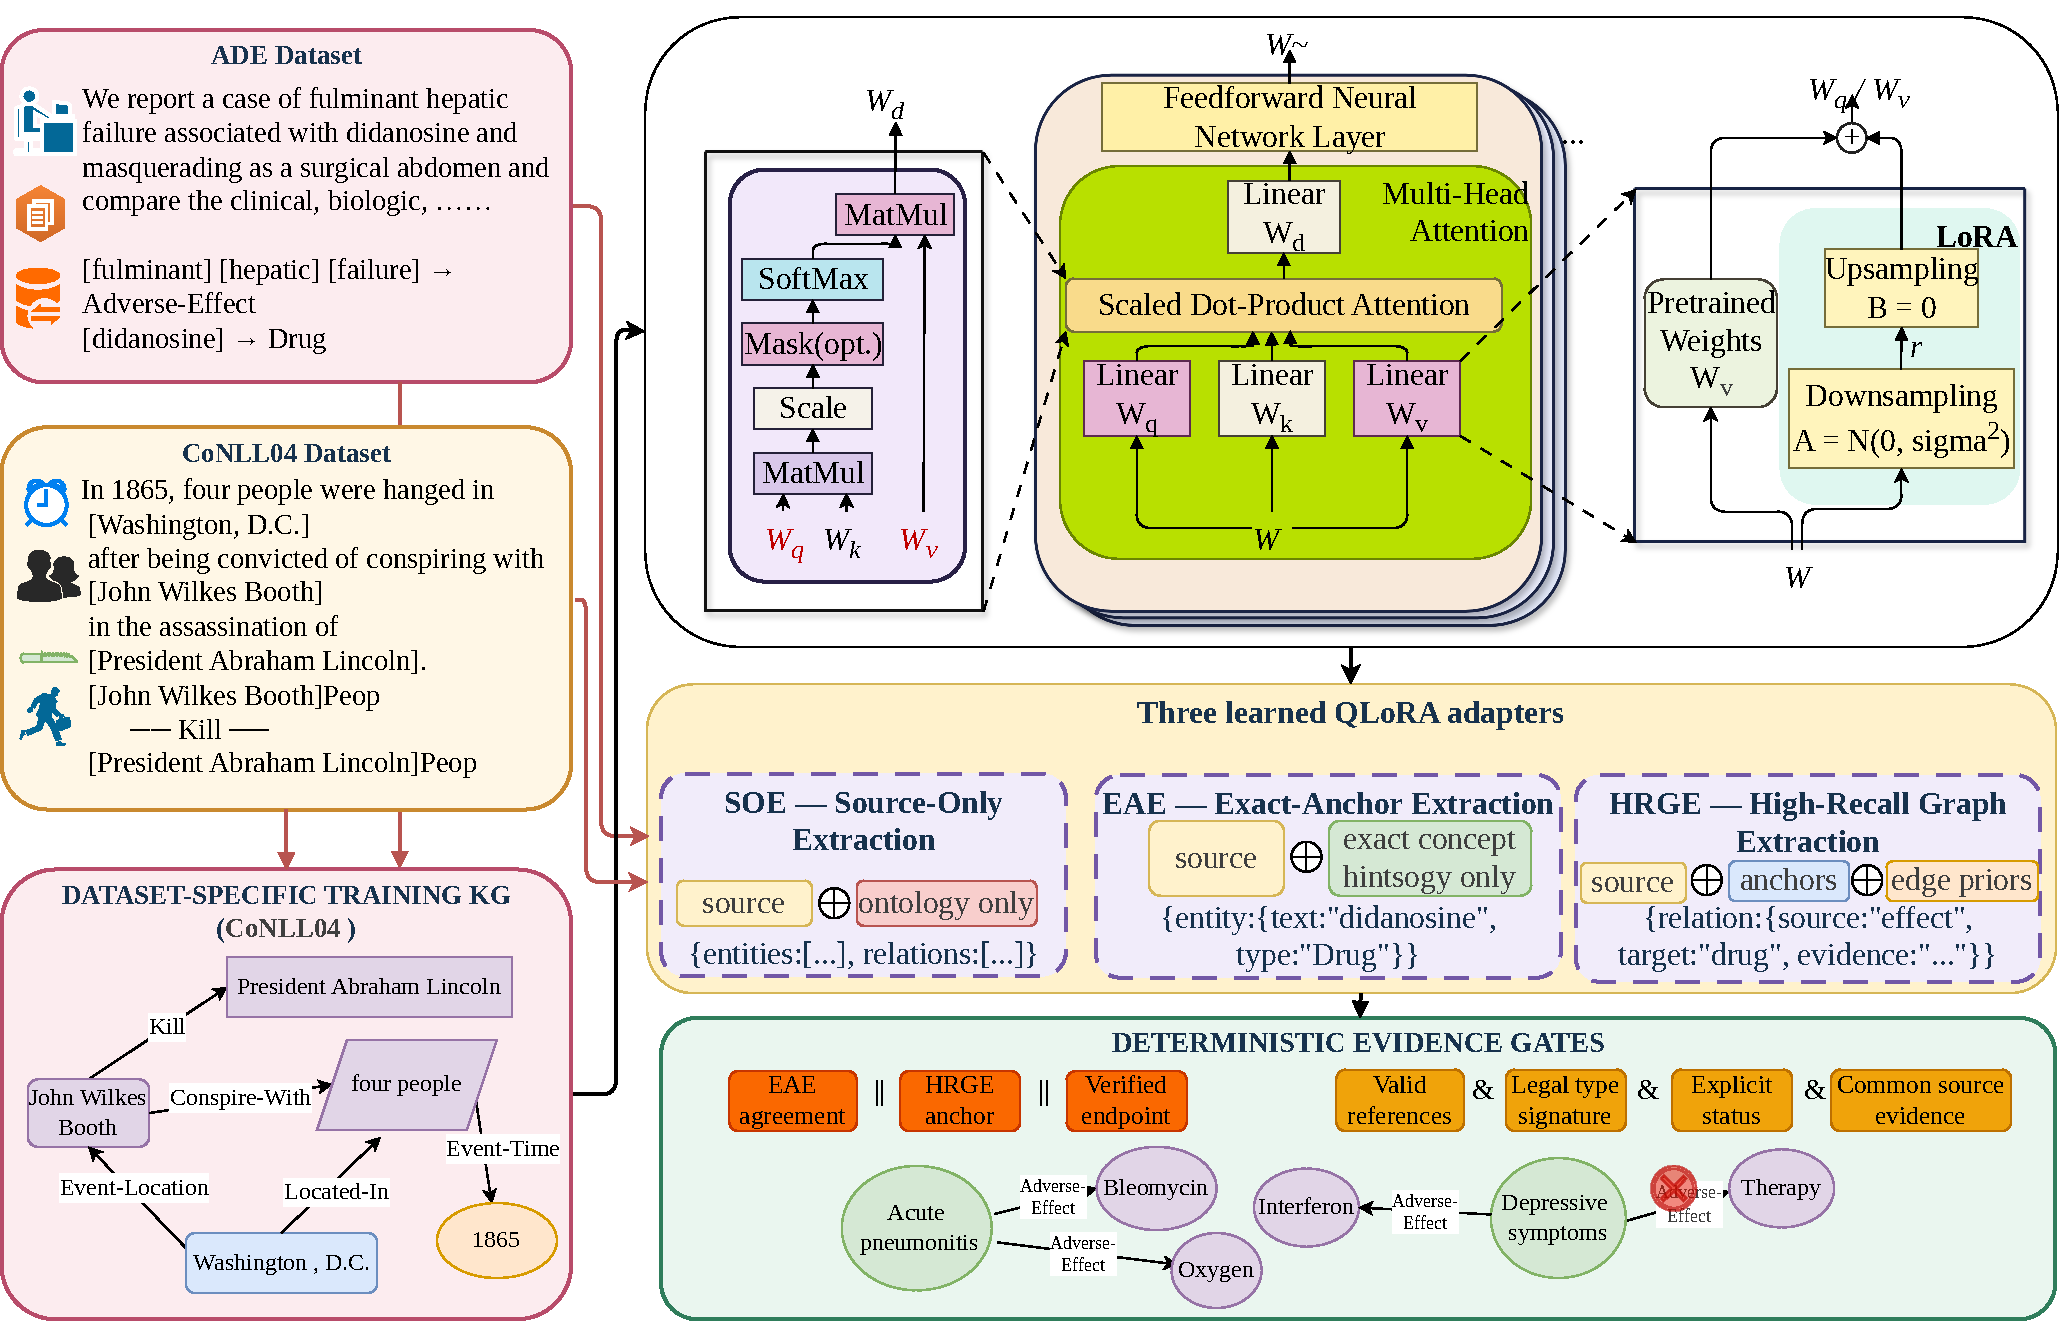
\includegraphics[width=\textwidth]{../figures/methodology.pdf}
\caption{本文的详细方法架构，包括 ADE 与 CoNLL04 输入、数据集专属训练知识图谱、Transformer 注意力模块、SOE/EAE/HRGE QLoRA 分支，以及基于一致性、锚点、端点、关系合法性和源证据的确定性门控。}
\label{zh:fig:architecture}
\end{figure*}

\subsection{来源受控的图谱上下文}
每个训练图谱存储提及字符串、类型、有向关系及支持它们的句子标识。若候选的唯一来源是当前训练句 $d$，该候选会被排除；若还有其他支持句，则保持可用。令 $\mathcal G_{\rm tr}=(\mathcal V_{\rm tr},\mathcal A_{\rm tr})$ 为只由训练标注构建的图，$\pi(c)$ 为上下文项 $c$ 的支持句标识集合，则训练样本 $i$ 的可用池为
\begin{equation}
\mathcal C_i^{\rm elig}
=\{c\in\mathcal C_i^{\rm raw}:\pi(c)\setminus\{i\}\neq\varnothing\}.
\label{zh:eq:provenance}
\end{equation}
该规则排除仅由当前样本支持的提示，但不声称对聚合统计执行了完全留一重算。评估标识与训练标识分离；精确文本重叠由更严格的隔离规则处理，即清空整个图谱上下文。

EAE 使用类型平衡的精确匹配概念提示。HRGE 使用三类上下文：通过类型纯度和提及形式过滤的源匹配锚点；要求存在当前样本之外支持且两个端点都出现在源句中的类型化边先验；以及由冻结 BGE-M3 检索的语义关系模式。设 $\mathbf H$ 为规范化候选记录向量，$\mathbf q$ 为规范化源句向量，则
\begin{equation}
\mathbf{s}=\mathbf{H}\mathbf{q},\qquad
\mathcal I=\operatorname{TopK}_{k}\{i:s_i\geq\tau\}.
\label{zh:eq:retrieval}
\end{equation}
该式只负责候选排序，不负责事实接受。检索上限和阈值固定于协议文件，提示也明确说明检索对象仅为线索；精确重叠隔离具有最高优先级。

\subsection{结构化生成与跨度重建}
生成器输出实体标识、复制文本和类型，以及关系标识、有向端点引用、关系类型与显式状态。模型不直接计算偏移。确定性展开程序把复制的提及分配到输入句中的实际出现位置，重建字符跨度，并记录无法匹配的字符串和无效引用。这样可以把语言模型候选生成与源坐标管理分开。

推理始终使用完整的输入句和固定生成策略。失败任务以空预测计入分母，而不会被删除。实验不采用依赖标注的补救窗口或按标签选择的句子截断。

\subsection{QLoRA 适配与训练目标}
三个生成分支均在相同的冻结 Qwen3-4B 骨干上采用匹配的 QLoRA 配置进行适配，低秩更新应用于注意力和前馈投影。对第 $\ell$ 个投影，有
\begin{equation}
W_{\ell}=W_{\ell}^{(0)}+\frac{\alpha}{r}B_{\ell}A_{\ell},
\qquad \operatorname{rank}(B_{\ell}A_{\ell})\leq r,
\label{zh:eq:qlora}
\end{equation}
其中 $W_{\ell}^{(0)}$ 是冻结量化权重，$r$ 为适配器秩，$A_{\ell}$ 和 $B_{\ell}$ 是可训练低秩因子。设 $y_{1:T}$ 是序列化目标，目标 token 的 $\omega_t=1$，提示 token 的 $\omega_t=0$，则优化目标为
\begin{equation}
\mathcal L(\theta)
=-\frac{1}{\sum_{t=1}^{T}\omega_t}
\sum_{t=1}^{T}\omega_t
\log p_{\theta}(y_t\mid y_{<t},x,\mathcal C).
\label{zh:eq:objective}
\end{equation}
提示 token 因而不参与损失。所有分支和重复运行使用相同数据划分与优化配置，完整参数保存在实验清单中。

\subsection{来源感知的候选验证与融合}
对关系标签 $z$，训练标注定义允许的源类型集合 $S_z$ 和目标类型集合 $T_z$。实现的类型约束为 $y_s\in S_z$ 且 $y_t\in T_z$，并不额外要求每个具体类型对都曾共同出现。综合引用、标签、端点类型、显式状态和源证据检查，关系谓词为
\begin{equation}
\begin{aligned}
V(r)={}&V_{\rm ref}(r)\land V_{\rm label}(r)\land V_{\rm type}(r)\\
&\land V_{\rm status}(r)\land V_{\rm evidence}(r).
\end{aligned}
\label{zh:eq:predicate}
\end{equation}
其中证据检查要求证据跨度有效，而且两个端点字符串同时位于一个源证据跨度内。验证关系集合为
\begin{equation}
R_V=\{r\in R_H:V(r)=1\}.
\label{zh:eq:verified}
\end{equation}
实体门控使用三个布尔信号：
\begin{equation}
A(e)=A_{\rm agree}(e)\lor A_{\rm anchor}(e)\lor A_{\rm endpoint}(e),
\label{zh:eq:accept}
\end{equation}
相应的接受实体集合为
\begin{equation}
E_A=\{e\in E_H:A(e)=1\}.
\label{zh:eq:accepted}
\end{equation}
一致性指 EAE 预测出相同的大小写折叠、空白规范化文本与类型；锚点支持要求存在同类型的源门控 HRGE 锚点；端点支持表示实体参与式\eqref{zh:eq:verified} 保留的关系。这三个信号互补但并非统计独立。句内重复的规范化文本--类型候选会被合并，关系只有在两个端点都保留时才能进入输出：
\begin{equation}
F(R,E)=\{(e_s,z,e_t)\in R:e_s\in E\land e_t\in E\}.
\label{zh:eq:endpoint}
\end{equation}
两种输出组合为
\begin{equation}
\begin{aligned}
G_{\rm CFE}&=(E_A,F(R_H,E_A)),\\
G_{\rm PGE}&=(E_A,F(R_V,E_A)).
\end{aligned}
\label{zh:eq:composition}
\end{equation}
系统记录每个接受或拒绝决定，使原始关系融合与验证关系融合的差异可直接审计。

\section{实验}
\subsection{实验设置}
实验在统一严格跨度协议下比较 PGE 与匹配的 SOE，并分析组件效应、训练行为、运行稳定性、规则合规性和精确重叠敏感性。双基准范围是聚焦的回顾性分析，而不是预注册的领域代表性抽样。模型与门控设置在报告的测试评估前固定，两次额外完整训练仅提供有限稳定性检查。

\subsubsection{数据集、标签与划分控制}
本文使用 SpERT 格式发布的句级 ADE 和 CoNLL04 文件。CoNLL04 保留原训练、开发和测试划分。ADE 含 3845 个训练池句子与 427 个测试句子；依据固定标识规则从训练池划出 384 句作为开发集，剩余 3461 句用于训练。该划分不是依据验证性能选择，也不是文献中常见 ADE 多折结果的平均。

表\ref{zh:tab:data} 给出从实际导入文件重新计算的统计。软件中的 document 单位是一条基准句，而不是完整病例或新闻文章。两套数据均为英文，因此结果不支持多语言或跨语言结论。

\begin{table*}[t]
\centering\small
\caption{实际实验划分的数据清单。长度为重建源文本的空白分词数。}
\label{zh:tab:data}
\resizebox{\textwidth}{!}{\begin{tabular}{llrrrr}
\toprule
Dataset & Split & Sentences & Entities & Relations & Mean length \\
\midrule
ADE & train & 3461 & 8717 & 5470 & 21.17 \\
ADE & validation & 384 & 996 & 627 & 21.82 \\
ADE & test & 427 & 1126 & 724 & 21.24 \\
CoNLL04 & train & 922 & 3377 & 1283 & 28.77 \\
CoNLL04 & validation & 231 & 893 & 343 & 30.27 \\
CoNLL04 & test & 288 & 1079 & 422 & 28.94 \\
\bottomrule
\end{tabular}
}
\end{table*}

ADE 包含 \textsc{Drug} 与 \textsc{Adverse Effect} 实体和一个 \textsc{Adverse Effect} 关系；导入端点方向为“不良反应到药物”，本文不将其反转。CoNLL04 包含 \textsc{Location}、\textsc{Organization}、\textsc{Person} 和 \textsc{Other} 实体，以及五种有向关系。表\ref{zh:tab:labels} 列出各划分的精确标签数。ADE 的单关系类别减少了类间混淆，却没有消除端点识别、方向和错误配对问题，因而不能把其较高 F1 简单解释为药物安全推理更容易。

\begin{table*}[t]
\centering\small
\caption{导入文件中各划分的实体与关系标注数量。}
\label{zh:tab:labels}
\resizebox{\textwidth}{!}{\begin{tabular}{lllrrr}
\toprule
Dataset & Kind & Label & Train & Validation & Test \\
\midrule
ADE & Entity & ADVERSE EFFECT & 4631 & 529 & 616 \\
ADE & Entity & DRUG & 4086 & 467 & 510 \\
ADE & Relation & ADVERSE EFFECT & 5470 & 627 & 724 \\
CoNLL04 & Entity & LOCATION & 1219 & 322 & 427 \\
CoNLL04 & Entity & ORGANIZATION & 616 & 170 & 198 \\
CoNLL04 & Entity & OTHER & 455 & 118 & 133 \\
CoNLL04 & Entity & PERSON & 1087 & 283 & 321 \\
CoNLL04 & Relation & KILL & 179 & 42 & 47 \\
CoNLL04 & Relation & LIVE IN & 330 & 91 & 100 \\
CoNLL04 & Relation & LOCATED IN & 247 & 65 & 94 \\
CoNLL04 & Relation & ORGANIZATION BASED IN & 271 & 76 & 105 \\
CoNLL04 & Relation & WORK FOR & 256 & 69 & 76 \\
\bottomrule
\end{tabular}
}
\end{table*}

ADE 与 CoNLL04 训练句平均长度分别为 21.17 和 28.77，测试均值为 21.24 和 28.94；全划分最大长度分别为 97 和 118。这些是描述性的空白 token 数，不是 Qwen tokenizer 数。两套导入数据中的每句话都至少含一个标注关系，因此实验没有测量以无关句为主的开放部署流中的误报行为。

图\ref{zh:fig:data} 报告训练标签比例和各划分句长经验累积分布。CoNLL04 的句子总体更长，而同一数据集内训练、验证、测试曲线大体一致。

\begin{figure*}[t]
\centering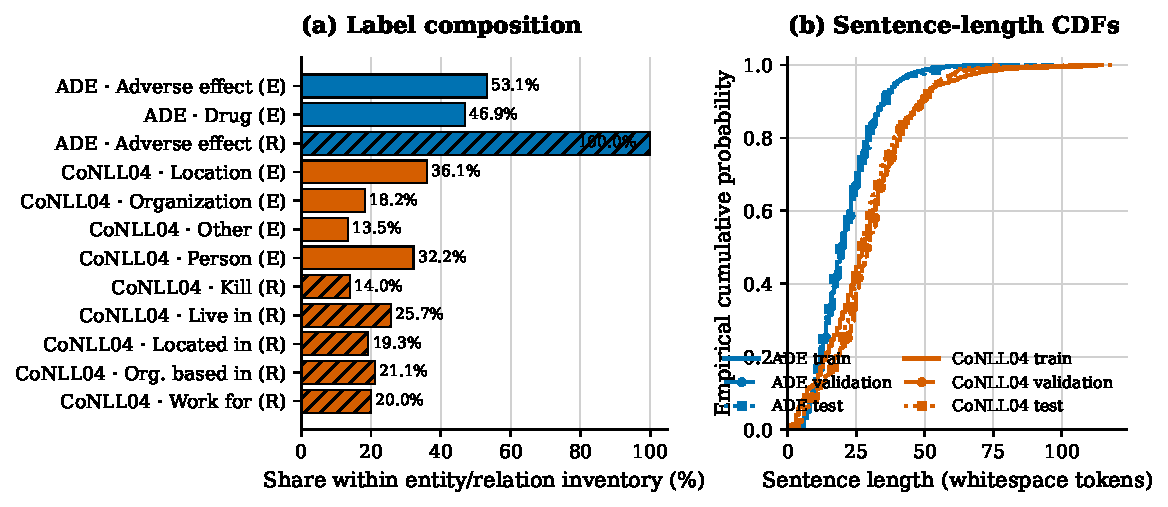
\includegraphics[width=\textwidth]{../figures/dataset_distribution.pdf}
\caption{数据分布分析。（a）各数据集实体（E）或关系（R）标签的训练集组成，各数据集--类别组合内部比例分别归一化为 100\%；（b）训练、验证和测试划分重建句长的经验累积分布，长度以空白 token 计。}
\label{zh:fig:data}
\end{figure*}

知识图谱按数据集分别构建，且只使用训练标注。对大小写折叠并压缩空白后的源字符串执行精确重叠检查：ADE 无训练--开发或训练--测试重叠；CoNLL04 有 14 个开发句和 19 个测试句与训练文本相同。系统在生成前清空这些句子的 EAE 与 HRGE 图谱上下文。由于这不能消除生成器训练时对重复文本的接触，本文另报告排除 19 个重叠测试句后的固定预测分析，但不声称检测了所有近重复或预训练污染。

\subsubsection{基线、指标与统计分析}
开发集比较含六个系统；测试表包含晋级的 SOE、PGE 和三种已完成外部比较。Qwen3-4B 零样本系统不使用本地适配，并接入记录的源展开与关系验证器；SpERT 在同一训练划分上从基础编码器训练；GLiNER+GLiREL 使用预测实体和仅训练集校准。这些是异构配置，而不是等算力实验。

所有主表预测由同一个公开字符跨度评估器重新评分。实体键包含精确源区间和类型，关系键包含两个类型化有向实体键和关系标签。证据偏移必须解析到源文本；重复键只计一次，无效对象作为未匹配预测，缺失任务作为空输出。池化计数为
\begin{equation}
\begin{aligned}
P&=\frac{TP}{TP+FP},\\
R&=\frac{TP}{TP+FN},\\
F_1&=\frac{2TP}{2TP+FP+FN}.
\end{aligned}
\label{zh:eq:metrics}
\end{equation}
式\eqref{zh:eq:metrics} 在每个数据集的句子间汇总，而不是平均逐句 F1。

统计分析对固定预测进行测试句配对 bootstrap，并在每次重采样中重算池化 F1。百分位区间描述已完成模型对的句子抽样不确定性，不表示训练重复变异，也不用于调整模型或门控。两次追加训练报告严格跨度 F1 的算术均值与样本标准差；由于 $n=2$，它只能展示观察到的初始化敏感性。seed-42 的 EAE/HRGE 日志每五个优化步记录一次损失，后续重复只有终点汇总，因此不进入损失曲线。合规计数基于评估器去重前的预测对象；重叠敏感性仅从两个系统同时删除相同测试标识，不重新训练或生成。

\subsection{主要结果}
表\ref{zh:tab:test} 给出统一评估器下的测试结果。ADE 上，PGE 把关系精确率从 80.62\% 提升到 87.00\%，召回率从 67.82\% 提升到 72.10\%，关系 F1 从 SOE 的 73.67\% 提升到 78.85\%；实体 F1 基本不变（87.97\% 对 87.93\%）。CoNLL04 上，关系精确率由 54.61\% 升至 62.40\%，召回率由 56.16\% 升至 57.82\%，关系 F1 由 55.37\% 升至 60.02\%，但实体 F1 由 83.83\% 降至 83.20\%。主要变化因此集中在关系，而不是全面改善提及识别。

\begin{table*}[t]
\centering\scriptsize
\caption{严格源字符跨度下的测试比较（micro，\%）。Qwen3-ZS 为接入记录验证器的 Qwen3-4B 零样本系统，GLiNER+GLiREL 仅使用训练集校准；所有行均由同一评估器重新评分。}
\label{zh:tab:test}
\resizebox{\textwidth}{!}{\begin{tabular}{llrrrrrr}
\toprule
Dataset & System & Ent. P & Ent. R & Ent. F1 & Rel. P & Rel. R & Rel. F1 \\
\midrule
ADE & Qwen3-ZS + verifier & 63.83 & 63.32 & 63.58 & 39.36 & 22.24 & 28.42 \\
ADE & GLiNER + GLiREL & 79.30 & 64.65 & 71.23 & 60.31 & 43.23 & 50.36 \\
ADE & SOE & 92.21 & $\mathbf{84.10}\uparrow$ & $\mathbf{87.97}\uparrow$ & 80.62 & 67.82 & 73.67 \\
ADE & PGE & $\mathbf{92.89}\uparrow$ & 83.48 & 87.93 & $\mathbf{87.00}\uparrow$ & $\mathbf{72.10}\uparrow$ & $\mathbf{78.85}\uparrow$ \\
CoNLL04 & Qwen3-ZS + verifier & 48.78 & 53.94 & 51.23 & 30.92 & 19.19 & 23.68 \\
CoNLL04 & GLiNER + GLiREL & 60.78 & 14.37 & 23.24 & 13.79 & 3.79 & 5.95 \\
CoNLL04 & SOE & 85.83 & $\mathbf{81.93}\uparrow$ & $\mathbf{83.83}\uparrow$ & 54.61 & 56.16 & 55.37 \\
CoNLL04 & PGE & $\mathbf{86.04}\uparrow$ & 80.54 & 83.20 & $\mathbf{62.40}\uparrow$ & $\mathbf{57.82}\uparrow$ & $\mathbf{60.02}\uparrow$ \\
\bottomrule
\end{tabular}
}
\end{table*}

图\ref{zh:fig:results} 表明 PGE--SOE 的改善具有关系特异性：两个数据集的关系 F1 都增加，实体差异则接近零且其配对区间跨越零。SpERT 在已完成系统中仍具有最高实体/关系 F1：ADE 为 91.37\%/84.08\%，CoNLL04 为 89.02\%/69.72\%。因此 PGE 优于匹配的生成基线，却没有超过训练后的跨度模型。PGE 也优于记录的零样本和 GLiNER+GLiREL 流水线，但这一结论只适用于当前标签映射与校准。

\begin{figure*}[t]
\centering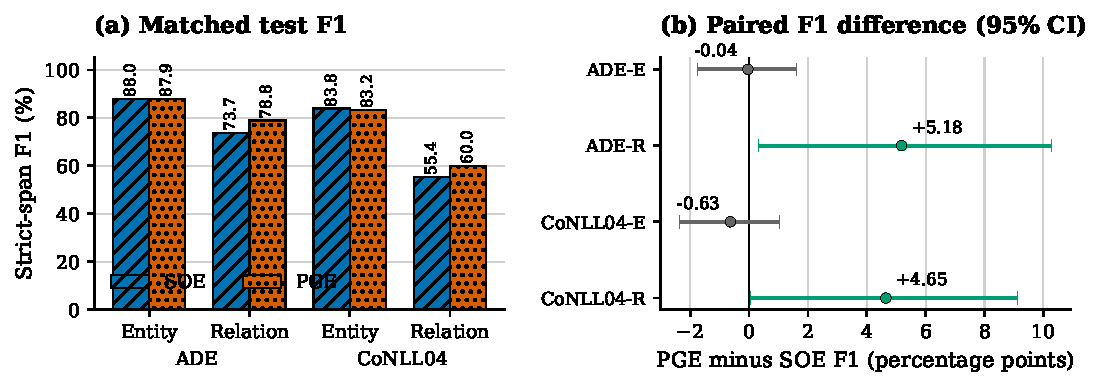
\includegraphics[width=\textwidth]{../figures/result_analysis.pdf}
\caption{匹配 SOE 与 PGE 的测试分析。（a）ADE 和 CoNLL04 上严格跨度实体与关系 F1；（b）PGE 减 SOE 的 F1 差异，水平区间为固定预测的配对 95\% 句子 bootstrap 区间。精确值和外部基线见表\ref{zh:tab:test}。}
\label{zh:fig:results}
\end{figure*}

\subsection{训练损失诊断}
图\ref{zh:fig:loss} 展示可追溯的 seed-42 EAE 与 HRGE 训练记录。浅色线是每五个优化步记录的原始值，强调线是十个记录点（50 个优化步）的尾随均值。CoNLL04 在单个 epoch 中明显下降；ADE 初始损失较低且噪声较大，只在后期轻微下降，不能描述为单调下降。SOE 和追加重复没有同等可归因的逐步历史，故不混入该诊断。

\begin{figure*}[t]
\centering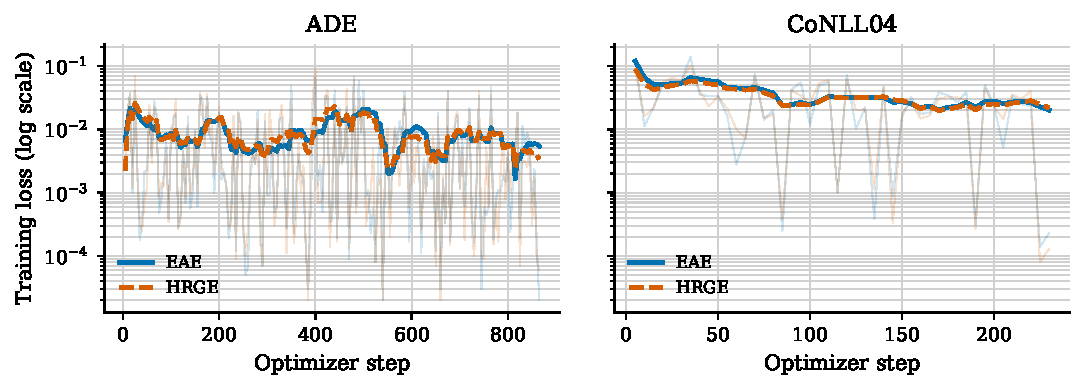
\includegraphics[width=\textwidth]{../figures/training_loss.pdf}
\caption{经审计的 seed-42 EAE 与 HRGE 适配器训练损失。原始观测每五个优化步写入运行日志，强调曲线为十个观测点的尾随均值；对数尺度保留原始波动，未重建或插值任何中间值。}
\label{zh:fig:loss}
\end{figure*}

\subsection{追加运行稳定性}
表\ref{zh:tab:runs} 汇总两次追加训练。ADE 上两次 PGE 关系 F1 均高于 SOE（81.20\% 对 78.31\%，80.62\% 对 78.06\%）；CoNLL04 的差异也为正但较小（58.50\% 对 56.91\%，61.45\% 对 60.92\%）。两次运行的平均关系 F1 差异在 ADE 和 CoNLL04 上分别为 2.73 与 1.06 个百分点。CoNLL04 实体 F1 平均下降 0.51 点，进一步说明观察到的是关系特异性而非普遍改善。

\begin{table*}[t]
\centering\small
\caption{统一严格跨度评估器下两次追加训练的测试稳定性（micro，\%，均值 $\pm$ 样本标准差，$n=2$）。末列为 PGE 减 SOE 的平均关系 F1。}
\label{zh:tab:runs}
\resizebox{\textwidth}{!}{\begin{tabular}{llrrr}
\toprule
Dataset & System & Entity F1 & Relation F1 & $\Delta$ relation F1 \\
\midrule
ADE & SOE & $88.00\pm0.37$ & $78.18\pm0.18$ & -- \\
ADE & PGE & $89.35\pm0.04$ & $80.91\pm0.41$ & $+2.73$ \\
CoNLL04 & SOE & $82.26\pm1.91$ & $58.92\pm2.84$ & -- \\
CoNLL04 & PGE & $81.75\pm2.02$ & $59.98\pm2.09$ & $+1.06$ \\
\bottomrule
\end{tabular}
}
\end{table*}

\subsection{配对差异与不确定性}
使用未四舍五入计数，ADE 的 PGE--SOE 关系 F1 差异为 5.18 个百分点，配对 95\% 区间为 [0.31, 10.29]；CoNLL04 差异为 4.65 点，区间为 [0.04, 9.12]。点估计与测试表一致，但区间较宽且下界接近零，只能解释为这些固定测试预测的证据，而不是跨训练运行保证。实体 F1 差异在 ADE 上为 $-0.04$（[$-1.75$, 1.62]），在 CoNLL04 上为 $-0.63$（[$-2.38$, 1.04]），均不支持实体性能提升。

\subsection{规则合规性分析}
测试 SOE 在 ADE 的 610 个关系对象中含 31 个规则无效对象，在 CoNLL04 的 436 个对象中含 16 个；PGE 分别保留 600 和 392 个关系对象，规则无效数均为零。HRGE 本身在 ADE 上为零，在 CoNLL04 的 413 个对象中只有 3 个无效对象，这区分了候选质量与验证器的贡献。

SOE、HRGE 和 PGE 在两个测试集上的测得无支持证据数均为零。由于关系证据被设为整句，一旦端点能够解析，共现条件较容易满足。因此，实验并没有展示“无支持断言率从非零降到零”，而是展示明确的证据绑定和规则合规；金标准 F1 则衡量预测类型化关系是否与标注一致，两者不能混同。

\subsection{精确重叠敏感性}
删除 19 个精确训练--测试重叠后，CoNLL04 剩余 269 个测试句、1023 个金标准实体和 403 个金标准关系。SOE 与 PGE 的关系 F1 分别为 53.79\% 和 59.10\%，差异为 5.31 点；实体 F1 分别为 83.02\% 和 82.90\%。关系优势在排除精确重叠后仍存在，但该分析不覆盖所有语义近重复或预训练污染。ADE 没有此类重叠，其敏感性结果与完整测试相同。

\subsection{消融实验}
表\ref{zh:tab:ablation} 在开发集上区分候选生成与确定性选择。ADE 上，HRGE 关系 F1 为 76.29\%，高于 SOE 的 73.16\%；EVGE 与 HRGE 相同，PGE 与 CFE 相同，说明这些变体中关系验证器未额外删除关系。实体门控降低 HRGE 召回，使 PGE 关系 F1 为 75.91\%，因此不能声称每个阶段都独立改善 F1。

CoNLL04 上，HRGE 关系 F1 为 58.26\%，低于 SOE 的 60.24\%；验证后为 59.60\%，最终 PGE 为 60.19\%，在开发集点估计上与 SOE 基本相同。门控提升实体精确率却降低召回率与 F1。本文保留开发与测试行为的差异，而不以测试结果反向选择消融版本。

\begin{table*}[t]
\centering\scriptsize
\caption{统一严格跨度评估器下的开发集消融（micro，\%）。这些系统用于刻画固定架构，并非额外晋级的测试系统。}
\label{zh:tab:ablation}
\resizebox{\textwidth}{!}{\begin{tabular}{llrrrrrr}
\toprule
Dataset & System & Ent. P & Ent. R & Ent. F1 & Rel. P & Rel. R & Rel. F1 \\
\midrule
ADE & SOE & 89.25 & 82.53 & 85.76 & 78.82 & 68.26 & 73.16 \\
ADE & EAE & 90.49 & 81.22 & 85.61 & 80.84 & 67.30 & 73.46 \\
ADE & HRGE & 90.35 & 85.54 & 87.88 & 80.04 & 72.89 & 76.29 \\
ADE & EVGE & 90.35 & 85.54 & 87.88 & 80.04 & 72.89 & 76.29 \\
ADE & CFE & 90.48 & 83.94 & 87.08 & 81.39 & 71.13 & 75.91 \\
ADE & PGE & 90.48 & 83.94 & 87.08 & 81.39 & 71.13 & 75.91 \\
CoNLL04 & SOE & 84.94 & 82.08 & 83.49 & 61.33 & 59.18 & 60.24 \\
CoNLL04 & EAE & 83.71 & 82.87 & 83.29 & 58.10 & 60.64 & 59.34 \\
CoNLL04 & HRGE & 82.35 & 81.52 & 81.94 & 60.06 & 56.56 & 58.26 \\
CoNLL04 & EVGE & 82.35 & 81.52 & 81.94 & 62.99 & 56.56 & 59.60 \\
CoNLL04 & CFE & 84.97 & 78.50 & 81.61 & 63.37 & 55.98 & 59.44 \\
CoNLL04 & PGE & 84.97 & 78.50 & 81.61 & 65.08 & 55.98 & 60.19 \\
\bottomrule
\end{tabular}
}
\end{table*}

\section{讨论}
\subsection{基准发现}
两个基准的共同结果是关系 F1 相对纯源文本生成提高。提升伴随关系精确率增加，而实体 F1 接近不变或略降，这与“治理候选接受”而非“扩大输出量”的设计目标一致。验证消融还显示图谱条件与选择规则相互作用：高召回上下文可以帮助 ADE，却不会自动改善 CoNLL04；当候选本身满足规则时，验证器也可能不发生作用。

数据分布有助于解释差异：ADE 训练规模更大、平均句子更短且只有一个关系类别；CoNLL04 训练句较少、输入更长且含五类关系。这些因素相互混杂而未被实验隔离，因此应按数据集分别报告，不能合并为单一因果解释。

回顾性收窄的双基准范围和少量追加训练限制了泛化。固定 ADE 划分不能直接与多折文献均值互换。两个语料都是英文且只含带关系句，无法证明多语言、长报告或开放流性能。缺乏上游文章标识时，句子 bootstrap 也不能恢复同一文章中句子间的依赖。

\subsection{可审计性}
系统公开了生成图谱对象的接受机制：图谱来源说明候选为何被建议，重建偏移说明它在源文本中的位置，门控记录说明为何保留或拒绝。这一优势属于架构层面；本文未开展用户研究来测量分析人员工作量、决策质量或信任，因此不能用规则完全合规替代这些证据。

门控也会付出覆盖率成本。一致性使用规范化文本--类型对，融合时可能合并重复提及，而评估器仍区分偏移，因而合法出现位置可能被删除。合法端点签名和句内共现不足以证明关系语义，三个门控信号也不是三次独立确认。因此最终结果仍应视为待人工复核的候选断言图。

精确重叠隔离阻止已知重复文本直接获得图谱提示，却不能消除生成器的训练暴露；预训练组件也可能见过相关材料。当前证据无法排除这种暴露。此外，分开的源类型集合与目标类型集合弱于观察到的联合类型对目录，后续可进一步收紧。

\subsection{安全相关意义}
ADE 将实验与药物安全信息抽取联系起来，CoNLL04 用于检验一般关系结构。框架可向分析人员同时呈现候选关系、源句、类型化端点和接受路径来源，供其接受、修改或拒绝。没有进入保留图谱并不意味着现实中的不良反应或其他关系不存在。

本文目标限于源链接抽取和证据路径检查。不同基线使用一个 epoch 生成式适配、20 个 epoch 的 SpERT 训练或预训练标签条件模型，训练日程并不相同。PGE 需要两个适配生成器和冻结检索，因此参数高效适配也不能被解释为已经证明的端到端成本节省。公开数据集或模型的可用性不自动授予所有再分发与商业使用权，仍应遵守原始许可证。

\section{结论与未来工作}
本文提出保持来源信息的证据门控图谱增强框架，并在 ADE 与 CoNLL04 上评估。统一严格跨度评估显示，PGE 相对 SOE 的关系 F1 分别提高 5.18 和 4.65 个百分点，同时提供显式、源链接的接受路径。排除 CoNLL04 精确训练--测试重叠后关系优势仍存在，两次追加运行也保持正差异，但 CoNLL04 的增益较小且实体性能没有提高。由此支持的结论是：受控图谱增强可以形成可审计的图谱引导抽取层，而不是对普遍准确率优势或语义真实性的保证。

未来应在预注册的多折划分、多语言与长文档语料、以及包含大量无关句的部署式数据流上检验框架。近重复聚类可扩展当前精确重叠分析，校准后的门控置信度与联合源--目标类型约束可改善精确率--覆盖率权衡。还需要更多训练重复、端到端延迟与资源测量，以及分析人员研究，才能判断可检查的接受路径是否确实降低复核成本或改善下游决策。

\section*{利益冲突声明}
作者声明不存在可能影响本文工作的已知竞争性经济利益或个人关系。

\section*{数据与代码可用性}
在合理请求下，可联系通信作者 Jingchao Wang 获取支持本研究结论的数据与代码。

\bibliographystyle{unsrtnat}
\bibliography{../cas-dc/references}
\end{document}
